% Schematic for the monotone lemma: a fixed block of area on [x,\lambda x].
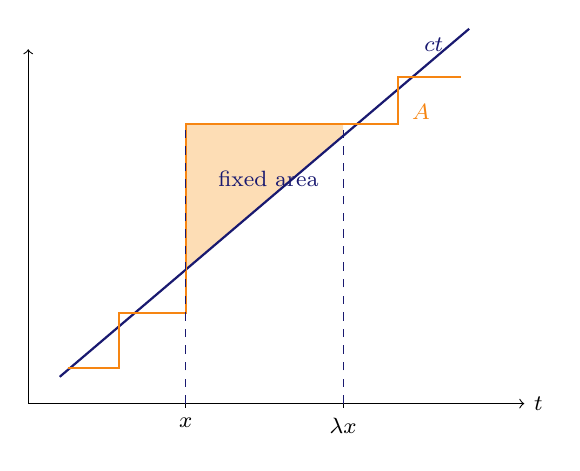
\begin{tikzpicture}[every node/.style={font=\footnotesize}]
  \draw[->] (0,0)--(6.3,0) node[right] {$t$};
  \draw[->] (0,0)--(0,4.5);
  \fill[BurntOrange!25] (2,1.7)--(4,3.4)--(4,3.55)--(2,3.55)--cycle;
  \draw[MidnightBlue,thick] (0.4,0.34)--(5.6,4.76);
  \node[MidnightBlue,above] at (5.15,4.35) {$ct$};
  \draw[BurntOrange,thick] (0.5,0.45)--(1.15,0.45)--(1.15,1.15)--(2,1.15)--(2,3.55)--(4.7,3.55)--(4.7,4.15)--(5.5,4.15);
  \draw[MidnightBlue,dashed] (2,0)--(2,3.55);
  \draw[MidnightBlue,dashed] (4,0)--(4,3.55);
  \draw (2,0)--(2,-0.06) node[below] {$x$};
  \draw (4,0)--(4,-0.06) node[below] {$\lambda x$};
  \node[BurntOrange,right] at (4.75,3.7) {$A$};
  \node[MidnightBlue] at (3.05,2.85) {fixed area};
\end{tikzpicture}
